%!TEX program=xelatex
% 注意事项:编译两次,以确保目录、页码完整显示
% 华东师范大学软件工程学院课程报告
% https://github.com/Shichien/ECNU-LateX-Template
% Author - 10235101526

\def\allfiles{}

\documentclass[14pt,a4paper,UTF8,twoside]{article}

% Title Page ————————————————————————————————————————
\usepackage{setspace}

% Formatting Packages ——————————————————————————————————————
\usepackage{multicol}
\usepackage{multirow}
\usepackage{enumitem}
\usepackage{indentfirst}

% Math & Physics Packages ————————————————————————————
\usepackage{amsmath, amsthm, amsfonts, amssymb}
\usepackage{physics}
\usepackage{cancel}
\usepackage{nicefrac}
\usepackage{unicode-math} % 允许数学公式使用特定字体
\usepackage{mdframed}
\usepackage{forest}

% Image-related Packages —————————————————————————————
\usepackage{float} % 浮动体环境
\usepackage{subcaption} % 子图包
\usepackage{pgfgantt}
\usepackage{graphics, graphicx}
\usepackage{tikz, tikz-qtree}
\usetikzlibrary{arrows.meta, positioning, fit, shapes}
\usetikzlibrary{shapes.geometric}
\tikzstyle{node_style} = [rectangle, rounded corners, draw, align=center, text width=3cm, minimum height=0.65cm]
\tikzstyle{arrow_style} = [thick, ->, >=stealth]

\usepackage{pgfplots}
\pgfplotsset{compat=1.18}
\usepackage{xcolor}
\usepackage{fourier-orns}
\usepackage{lipsum}

% Colour Palette ——————————————————————————————————————
\definecolor{merah}{HTML}{F4564E}
\definecolor{merahtua}{HTML}{89313E}
\definecolor{biru}{HTML}{60BBE5}
\definecolor{birutua}{HTML}{412F66}
\definecolor{hijau}{HTML}{59CC78}
\definecolor{hijautua}{HTML}{366D5B}
\definecolor{kuning}{HTML}{FFD56B}
\definecolor{jingga}{HTML}{FBA15F}
\definecolor{ungu}{HTML}{8C5FBF}
\definecolor{lavender}{HTML}{CBA5E8}
\definecolor{merjamb}{HTML}{FFB6E0}
\definecolor{mygray}{HTML}{E6E6E6}
\definecolor{mygreen}{rgb}{0,0.6,0}
\definecolor{mymauve}{rgb}{0.58,0,0.82}

% Theorems ————————————————————————————————————————————
\usepackage{tcolorbox}
\usepackage{changepage}
\tcbuselibrary{skins,breakable,theorems}

\newcounter{hitung}
\setcounter{hitung}{\thesection}

\makeatletter
% Proof 证明如下
\def\tcb@theo@widetitle#1#2#3{\hbox to \textwidth{\textsc{\large#1}\normalsize\space#3\hfil(#2)}}
\tcbset{
    theorem style/theorem wide name and number/.code={ \let\tcb@theo@title=\tcb@theo@widetitle},
    proofbox/.style={skin=enhancedmiddle,breakable,parbox=false,boxrule=0mm,
    check odd page, toggle left and right, colframe=black!20!white!92!hijau,
    leftrule=8pt, rightrule=0mm, boxsep=0mm,arc=0mm, outer arc=0mm,
    left=3mm,right=3mm,top=0mm,bottom=0mm, toptitle=0mm,
    bottomtitle=0mm,colback=gray!3!white!98!biru, before skip=8pt, after skip=8pt,
    before={\par\vskip-2pt},after={\par\smallbreak},
    },
}
\newtcolorbox{ProofBox}{proofbox}
\makeatother

\let\realproof\proof
\let\realendproof\endproof
\renewenvironment{proof}[1][Prove:]{\ProofBox\strut\textsc{#1}\space}{\endProofBox}
\AtEndEnvironment{proof}{\null\hfill$\blacksquare$}

% Example
\newtcolorbox[use counter=hitung, number within=section]{Thought}[1][]{breakable,
    colframe=white!10!jingga, coltitle=white!90!jingga, colback=white!85!jingga, coltext=black!10!brown!50!jingga, colbacktitle=white!10!jingga, enhanced, fonttitle=\bfseries,fontupper=\normalsize, attach boxed title to top left={yshift=-2mm}, before skip=8pt, after skip=8pt,
    title=Thought \ \ #1}

%% Komentar/Remark
\newtcolorbox{rmr}[1][]{
    arc=0mm, outer arc=0mm,
    boxrule=0pt, toprule=1pt, leftrule=0pt, bottomrule=5pt, rightrule=0pt,
    left=0.2cm, right=0.2cm,
    titlerule=0.5em, toptitle=0.1cm, bottomtitle=-0.1cm, top=0.2cm,
    colframe=white!10!kuning, % 边框颜色
    colback=white!85!kuning,  % 背景颜色
    coltitle=white!30!black,         % 标题颜色
    coltext=orange!60!kuning,          % 文字颜色
    fonttitle=\bfseries, fontupper=\normalsize,
    before skip=8pt, after skip=8pt,
    title=提示: #1
}

% Catatan/Note
\newtcolorbox{note}[1][]{enhanced,
    left=4.1mm, borderline west={8pt}{0pt}{white!10!kuning},
    before skip=6pt, after skip=6pt,
    colback=white!85!kuning, colframe= white!85!kuning, coltitle=orange!60!kuning!25!brown, coltext=orange!60!kuning!25!brown,
    fonttitle=\bfseries,fontupper=\normalsize, before skip=8pt, after skip=8pt,
    title=Note\underline{}  #1}


\usepackage{booktabs} % 表格库
\usepackage{titlesec} % 标题库
\usepackage{fancyhdr} % 页眉页脚库
\usepackage[sorting=none]{biblatex}
\usepackage{array}

\date{} % 留空,以让编译时去除日期

%———————————————注意事项—————————————————%

% 1、如果编译显示失败,但没有错误信息,就是 filename.pdf 正在被占用
% 2、在文件夹中的终端使用 Windows > xelatex filename.tex 也可编译

%—————————————华东师范大学———————————————%

% 论文制作时须加页眉,页眉从中文摘要开始至论文末
% 偶数页码内容为:华东师范大学硕士学位论文,奇数页码内容为学位论文题目

%————————定义 \section 的标题样式————————%

% 注意:\chapter 等命令,内部使用的是 \thispagestyle{plain} 的排版格式
% 若需要自己加上页眉,实际是在用 \thispagestyle{fancy} 的排版格式
% 加上下面这一段指令,就能够让 \section 也使用 fancy 的排版格式
% 本质就是让目录、第一页也能够显示页眉、页脚

\fancypagestyle{plain}{
    \pagestyle{fancy}
}

\title{华东师范大学软件学院课程报告} % 模板
\titleformat{\section}
{\normalfont\bfseries\Large} % 字体大小、字体系列(\bfseries 为加粗)
{\thesection}{1em}{}

% ———————————设置章节的中文格式———————————%
\renewcommand\thesection{\chinese{section} \hspace{0pt}}
\renewcommand\thesubsection{\arabic{subsection} \hspace{0pt}}
% \renewcommand\thesubsubsection{\alph{subsubsection} \hspace{0pt}} % 字母编号
% \hspace{0pt} 是为了确保在章节编号和章节题目之间不要有空格,使得排版更为美观

%—————————————页面基础设置———————————————%

\usepackage{geometry}
\geometry{left=10mm, right=10mm, top=20mm, bottom=20mm}

%————————————设置页眉、页脚——————————————%

\pagestyle{fancy} % 设置 plain style 的属性

% 设置页眉

\fancyhead[RE]{\footnotesize \leftmark} % Right Even 偶数页右侧显示章名 \leftmark 最高级别章名
\fancyhead[LO]{\footnotesize \rightmark} % Left Odd 奇数页左侧显示节名 \rightmark 第二级别节名
\fancyhead[C]{华东师范大学软件学院课程报告} % Center 居中显示
\fancyhead[LE,RO]{~\thepage~} % 在偶数页的左侧,奇数页的右侧显示页码
\renewcommand{\headrulewidth}{1.2pt} % 页眉与正文之间的水平线粗细

% 设置页脚:在每页的右下脚以斜体显示书名

\fancyfoot[RO,RE]{\it Project Report By \LaTeX} % 使用意大利斜体显示
\renewcommand{\footrulewidth}{0.5pt} % 页脚水平线宽度

%——————设置页码:在底部居中显示页码———————%

\usepackage{lastpage} % 页码数库
\pagestyle{fancy}
\fancyfoot[C]{\kaishu 第 \thepage 页 \ 共 \pageref{LastPage} 页} % LastPage 需要二次编译以获取总页数

%——————————————代码块设置———————————————%

\usepackage{listings} % 代码块包
\lstset {
    backgroundcolor=\color{white},   % choose the background color; you must add \usepackage{color} or \usepackage{xcolor}
    basicstyle=\ttfamily\footnotesize,        % the size of the fonts that are used for the code
    breakatwhitespace=false,         % sets if automatic breaks should only happen at whitespace
    breaklines=true,                 % sets automatic line breaking
    captionpos=bl,                   % sets the caption-position to bottom
    commentstyle=\color{mygreen},    % comment style
    deletekeywords={...},            % if you want to delete keywords from the given language
    escapeinside={\%*}{*},           % if you want to add LaTeX within your code
    extendedchars=true,              % lets you use non-ASCII characters; for 8-bits encodings only, does not work with UTF-8
    frame=single,                    % adds a frame around the code
    keepspaces=true,                 % keeps spaces in text, useful for keeping indentation of code (possibly needs columns=flexible)
    keywordstyle=\color{blue},       % keyword style
% language=Python,               % the language of the code
    morekeywords={*,...},            % if you want to add more keywords to the set
    numbers=left,                    % where to put the line-numbers; possible values are (none, left, right)
    numbersep=5pt,                   % how far the line-numbers are from the code
    numberstyle=\tiny\color{black}, % the style that is used for the line-numbers
    rulecolor=\color{black},         % if not set, the frame-color may be changed on line-breaks within not-black text (e.g. comments (green here))
    showspaces=false,                % show spaces everywhere adding particular underscores; it overrides 'showstringspaces'
    showstringspaces=false,          % underline spaces within strings only
    showtabs=false,                  % show tabs within strings adding particular underscores
    stepnumber=1,                    % the step between two line-numbers. If it's 1, each line will be numbered
    stringstyle=\color{orange},      % string literal style
    tabsize=2,                       % sets default tabsize to 2 spaces
% title=Python Code              % show the filename of files included with \lstinputlisting; also try caption instead of title
}

% 注释掉的部分用于后续插入代码,参数可调整,格式如下:

% 1、直接插入
% \begin{lstlisting}[language = ? , title = { ? } ]
%       Your code here.
% \end{lstlisting}

% 2、文件插入
% \lstinputlisting[language = C , title = ?.c] {filename.c}

%———————————————字体设置————————————————%

\usepackage{fontspec} % 允许设置字体
\usepackage[utf8]{inputenc}
\usepackage{ctex}
\linespread{1.2}
% \setCJKmainfont{SimSun} % 设置正文罗马族的 CJK 字体

% 定义新的命令,将所有 \texttt{} 包裹的内容变成蓝色
% \renewcommand{\texttt}[1]{{\color{blue}\ttfamily#1}}
\setmainfont{Consolas}


%———————————————超链接设置——————————————%

\usepackage[hidelinks]{hyperref}
\hypersetup{
    pdfstartview=FitH, % 设置PDF文档打开时的初始视图为页面宽度适应窗口宽度(即页面水平适应)
    CJKbookmarks=true, % 用对CJK(中文、日文、韩文)字符的书签支持,确保这些字符在书签中正确显示
    bookmarksnumbered=true, % 书签带有章节编号。这对有章节编号的文档很有用
    bookmarksopen=true, % 文档打开时,书签树是展开的,方便查看所有书签
%    colorlinks, % 启用彩色链接。这样,链接在PDF中会显示为彩色,而不是默认的方框
    pdfborder=001, % 设置PDF文档中链接的边框样式。001 表示链接周围没有边框,仅在单击时显示一个矩形
%    linkcolor=blue, % 设置文档内部链接(如目录中的章节链接)的颜色为蓝色
%    anchorcolor=blue, % 设置锚点链接(即目标在同一文档内的链接)的颜色为蓝色
%    citecolor=blue, % 设置引用(如文献引用)的颜色为蓝色
}

%——————————————导言区结束,进入正文部分———————————————%

\begin{document}

    \begin{titlepage}
        \centering
        \vspace*{2cm}

        
\includegraphics[width=0.6\textwidth]{img/ECNULogo}\par\vspace{1cm}

        {\heiti \zihao{-1} ECNU 校园插件项目报告}\\[1.5cm]

        {\bfseries\zihao{-1} ECNU Campus Plugins - Project Report}\\[1.5cm]

        {\kaishu \zihao{2} 关卓谦 \ \ 张梓卫 \ \ 王文锦}\\[1cm]

        {\zihao{3} 指导老师:陈良育}\\[1cm]

        \vfill

        {\zihao{3} \today}

        \vspace{1cm}

        {\zihao{3} 华东师范大学软件工程专业}

    \end{titlepage}

    \newpage{}

    \tableofcontents

    \newpage{}


    \section{项目概述}

    \subsection{项目背景}

    本项目旨在为 ECNU 校园提供支持,专注于解决校园生活中的痛点,并通过自动化功能提升便利性与体验。

    \subsection{项目信息}

    \begin{itemize}
        \item 项目作者:关卓谦(10235101529)、张梓卫(10235101526)、王文锦(10235101510)
        \item 项目仓库(含部署方法及 Wiki 文档):\href{https://github.com/azazo1/ecnu-campus-plugins}{\underline{https://github.com/azazo1/ecnu-campus-plugins}}
        \item 本项目遵循 MIT 开源协议,供感兴趣者学习和交流。
        \item 华东师范大学校徽图案版权归华东师范大学所有。
        \item 本项目使用 Python 3.12 开发,使用 Pyside 6 实现图形界面。
    \end{itemize}

    \subsection{项目功能}

    \begin{tcolorbox}[
        theorem style=theorem wide name and number,breakable,enhanced,arc=3.5mm,outer arc=3.5mm,
        boxrule=0pt,toprule=1pt,leftrule=0pt,bottomrule=1pt, rightrule=0pt,left=0.2cm,right=0.2cm,
        titlerule=0.5em,toptitle=0.1cm,bottomtitle=-0.1cm,top=0.2cm,
        colframe=white!10!hijau,colback=white!90!hijau,coltitle=white, coltext=hijautua!80!brown,
        shadow={1.3mm}{-1.3mm}{0mm}{gray!50!white}, % 添加阴影
        title style={white!10!hijau}, before skip=8pt, after skip=8pt,
        fonttitle=\bfseries,fontupper=\normalsize,
        title={本项目包含:}
    ]
        \begin{itemize}
            \item 一键生成当周课表、课前邮件提醒
            \item 课后研修间与图书馆的全自动预约
            \item 宿舍电费自动查询及充值提醒
        \end{itemize}
    \end{tcolorbox}


    \section{项目结构}\label{sec:project-structure}

    \begin{center}
        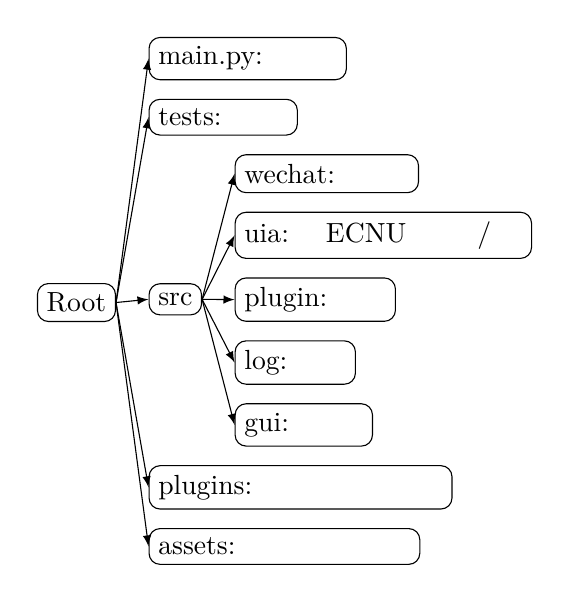
\begin{tikzpicture}
            % 绘制项目结构的树状图
            \node at (0, 0) {
                \begin{forest}
                    for tree={
                        grow=east,
                        draw,
                        edge={-latex},
                        rounded corners,
                        node options={align=center},
                        anchor=west,
                        parent anchor=east,
                        child anchor=west,
                        delay={where content={}{shape=coordinate}{}} % 避免错误节点
                    }
                    % @formatter:off
                    [Root
                        [assets: 静态资源目录,包含各开发参考文件及图标等。]
                        [plugins: 各个插件具体实现,可单独删除和添加、启动和停止
                            % todo 记得填写插件一句话简介
                        ]
                        [src
                            [gui: 实现图形用户界面]
                            [log: 实现日志输出]
                            [plugin: 实现插件架构]
                            [uia: 实现 ECNU 统一身份认证辅助/自动登录]
                            [wechat: 实现微信自动控制]
                        ]
                        [tests: 项目早期测试集]
                        [main.py: 软件启动入口文件]
                    ]
                    % @formatter:on
                \end{forest}
            };
        \end{tikzpicture}
    \end{center}

    \section{项目详述}\label{sec:project-desc}

    \subsection{插件登录 ECNU 及辅助登录}\label{subsec:plugin-login-ecnu}
    插件许多功能需要调用 ECNU 提供的各种接口。
接口的调用依赖于 ECNU 各个系统的登录缓存(在项目内部保存为 \verb`LoginCache`)。
为了获取有效的登录缓存简化登录操作,
插件登录使用了 WebDriver 控制浏览器实现自动化或半自动化的辅助登录流程。

在插件登录时,会出现浏览器 ECNU 统一身份认证的界面,登录有两种方式。
\begin{itemize}
    \item 方法一:填写图\ref{fig:uia-login-form} 中的表单实现登录。
    \item 方法二:扫描图\ref{fig:uia-login-qrcode} 中的二维码实现登录。
\end{itemize}

\begin{table}[H]
    \centering
    \begin{tabular}{cc}
        \begin{minipage}[H]{0.5\textwidth}
            \centering
            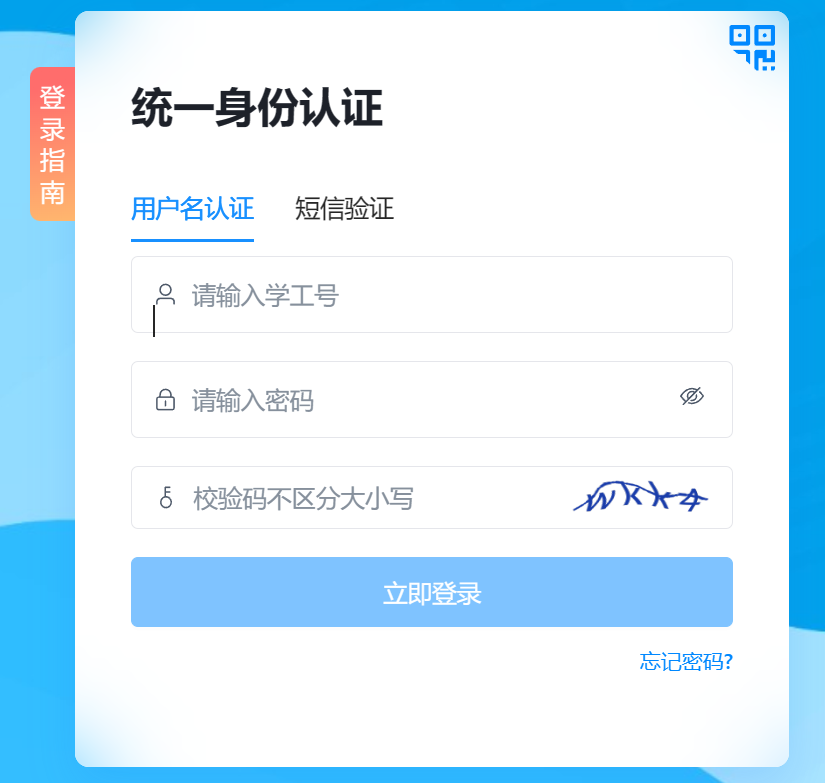
\includegraphics[width=0.8\textwidth]{img/uia_login_form}
            \captionof{figure}{ECNU UIA 登录界面(表单)}
            \label{fig:uia-login-form}
        \end{minipage} &
        \begin{minipage}[H]{0.5\textwidth}
            \centering
            
\includegraphics[width=0.8\textwidth]{img/uia_login_qrcode}
            \captionof{figure}{ECNU UIA 登录界面(二维码)}
            \label{fig:uia-login-qrcode}
        \end{minipage}
    \end{tabular}
\end{table}

\begin{rmr}[切换表单登录和二维码登录]
    \quad 表单登录:
    可以在项目根目录创建文件 \verb`login_info.toml`
    然后填写如下内容(替换尖括号以内的部分)。
    插件登录时会读取此文件中的学号密码,自动填写图\ref{fig:uia-login-form} 中的表单,实现全自动辅助登录。
    % @formatter:off
    \begin{verbatim}
stu_number = "<填写学号>"
password = "<填写数据库密码>" \end{verbatim}
    % @formatter:on

    \quad 二维码登录:
    删除 \verb`login_info.toml` 文件,
    此时插件辅助登录时会截取二维码图片并发送至邮箱提醒(如果已配置 \verb`email_notifier` 插件,见\ref{plugin-email-notifier})。 % todo 完成这个插件的介绍
    可以使用微信扫描二维码或用微信打开邮件中的连接实现半自动登录。
\end{rmr}

\subsubsection{辅助登录大致实现}

当此软件执行辅助登录的时候:

\begin{description}
    \item[二维码登录]
    进入 ECNU 统一身份认证(下面简称 UIA)界面之后,辅助登录默认使用二维码登录而不是表单登录。
    二维码登录时,脚本截取 UIA 二维码登录图片然后发送到目标邮箱,通过用户微信扫描二维码或者微信打开邮箱中的连接来实现登录。
    \item[表单登录]
    如果创建了 \verb`login_info.toml` 文件(步骤见上述提示),那么脚本会读取其中的学号和密码并自动填写到 UIA 表单中。
    表单中的验证码通过开源库 \hyperref{https://github.com/sml2h3/ddddocr}{DDDDocr} 来识别,成功识别四位验证码之后模拟点击登录按钮来登录。
    如果验证码识别失败则刷新重试。
\end{description}

成功登录 UIA 之后,各个插件通过自己实现的缓存抓取函数(\textit{Cache Grabber})在各个 ECNU 系统中获得所需要的登录缓存。

最终,登录缓存通过插件加载器(\textit{Plugin Loader})分发给各个插件。

    \subsection{插件框架}\label{subsec:plugin-framework}
    为了合理地分离代码中的各个逻辑部分,项目构建了插件框架,将不同的功能划分到一个个插件中。
插件框架实现了单独开启和关闭每个插件的功能,让使用者可以根据需要选择希望使用的功能。

插件框架的大致内容如下:

\subsubsection{插件加载器(PluginLoader)}
插件的加载和运行通过 PluginLoader 来驱动。

项目启动时,PluginLoader 依次导入位于项目根目录下的 \verb`plugins` 文件夹中的插件。
然后从文件中读取各个插件配置,并传递给插件。
插件配置读取完毕之后,PluginLoader 加载各个插件。
被加载的插件可以从其他插件中接收消息和按照特定周期执行(\ref{para:routine})。

\subsubsection{插件注册(Register)}
插件注册无需直接与 PluginLoader 进行交互。
插件加载器会在项目启动的时候自动导入 plugins 文件夹下的每个 \verb`python` 包或者一个 \verb`.py` 文件,
并尝试注册其中的插件。

插件的注册通过装饰器 \verb`register_plugin` 进行。
继承插件类并通过 \verb`register_plugin` 即可注册插件:

% @formatter:off
\begin{lstlisting}[
    language={Python},
    caption={插件注册代码示例},
    captionpos=b,
    label=lst:plugin-registering,
]
@register_plugin(
    name="demo_plugin"
)
class DemoPlugin(Plugin):
    pass\end{lstlisting}
% @formatter:on

\subsubsection{插件事件方法}

成功注册后插件的各种事件方法会被触发,主要的事件方法如下。

\paragraph{插件加载和停止(Load 与 Unload)事件}

当插件被加载和停止时触发,插件的加载和停止在插件被导入之后,可能会被使用者多次触发。
用于标记当前插件是否正在运行,方便插件释放资源。


% @formatter:off
\begin{lstlisting}[
    language={Python},
    caption={插件加载和停止示例},
    captionpos=b,
    label=lst:plugin-load-unload,
]
@register_plugin(
    name="demo_plugin"
)
class DemoPlugin(Plugin):
    def on_load(self, ctx: PluginContext):
        pass
    def on_unload(self, ctx: PluginContext):
        pass\end{lstlisting}
% @formatter:on

\paragraph{插件周期事件(Routine)}\label{para:routine}
插件在注册的时候可以提供一个回调周期,插件会在指定的回调周期得到回调。

% @formatter:off
\begin{lstlisting}[
    language={Python},
    caption={插件周期事件示例},
    captionpos=b,
    label=lst:plugin-routine,
]
@register_plugin(
    name="demo_plugin",
    routine=Routine.MINUTELY
)
class DemoPlugin(Plugin):
    def on_routine(self, ctx: PluginContext):
        pass # 周期性得到回调\end{lstlisting}
% @formatter:on

\subsubsection{插件配置(PluginConfig)}
插件在插件注册时提供需要的配置,在 PluginLoader 从文件中读取插件配置的时候,获得配置的值。

插件配置会集中保存在 \verb`plugin_config.toml` 中,gui
会为每个插件配置自动生成交互式修改组件,见\ref{subsubsec:gui-plugin-config}。
使用者可以通过修改文件或者通过 gui 修改插件配置。

% @formatter:off
\begin{lstlisting}[
    language={Python},
    caption={插件配置示例},
    captionpos=b,
    label=lst:plugin-config,
]
@register_plugin(
    name="demo_plugin",
    configuration=PluginConfig()
    .add(TextItem(name="first_name", default_value="Tom", description="Your first name"))
)
class DemoPlugin(Plugin):
    def on_config_load(self, ctx: PluginContext, cfg: PluginConfig):
        first_name = cfg.get_itme("first_name").current_value\end{lstlisting}
% @formatter:on

\subsubsection{插件缓存(PluginCache)}
插件内部生成的数据可以得到统一的持久化保存。
插件只需对 PluginCache,进行修改,数据会在插件停止时保存,在插件加载时再次读取。

% @formatter:off
\begin{lstlisting}[
    language={Python},
    caption={插件缓存示例},
    captionpos=b,
    label=lst:plugin-cache,
]
@register_plugin(
    name="demo_plugin"
)
class DemoPlugin(Plugin):
    def on_load(self, ctx: PluginContext):
        ctx.get_logger().info(ctx.get_cache().get("time"))
    def on_routine(self, ctx: PluginContext):
        ctx.get_cache().set("time", time.time())\end{lstlisting}
% @formatter:on

\subsubsection{插件上下文(PluginContext)}
插件上下文为插件提供多种间接与项目交互的方式。

插件可以通过 PluginContext 进行
\begin{enumerate}
    \item 输出日志
    \item 创建可交互按钮(Bind Action)
    \item 读写缓存
    \item 向其他插件发送消息
    \item 获取登录缓存
\end{enumerate}
等操作。

\subsubsection{插件消息传递(Message)}
插件通过 PluginContext 可以向其他插件发送消息。

% @formatter:off
\begin{lstlisting}[
    language={Python},
    caption={插件发送消息示例},
    captionpos=b,
    label=lst:plugin-send-message,
]
@register_plugin(
    name="send_demo_plugin"
)
class DemoPlugin(Plugin):
    def on_routine(self, ctx: PluginContext):
        ctx.send_message("recv_demo_plugin", "Hello World")

@register_plugin(
    name="recv_demo_plugin"
)
class RecvPlugin(Plugin):
    def on_recv(self, ctx: PluginContext, from_plugin: str, obj: Any):
        ctx.get_logger().info((from_plugin, obj))\end{lstlisting}
% @formatter:on


    \subsection{插件}\label{subsec:plugins}
    \subsubsection{研修间预约插件}

% todo 介绍插件主要功能
    \subsubsection{图书馆预约插件}

% todo 介绍插件主要功能
    \subsection{课前提醒模块} % todo subsub

\subsubsection{代码框架及分析}

\subsubsection{课表获取及数据处理原理}

\begin{table}[H]
    \centering
    \begin{tabular}{cc}
        \begin{minipage}[H]{0.4\textwidth}
            \centering
            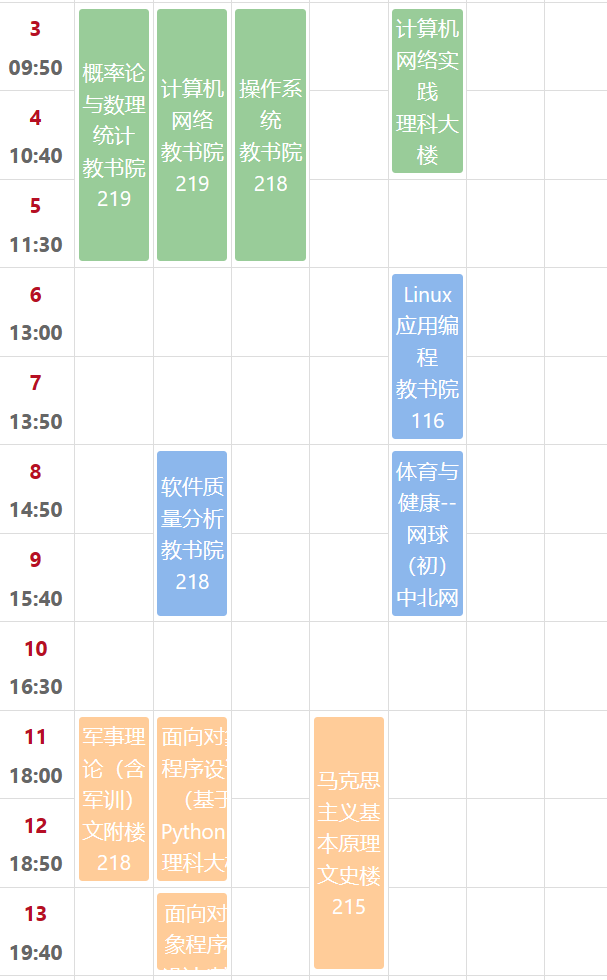
\includegraphics[width=0.5\textwidth]{img/calendar.png}
            \captionof{figure}{ECNU Portal 课表页面}
            \label{fig:login}
        \end{minipage} &
        \begin{minipage}[H]{0.5\textwidth}
            \raggedright
            \begin{rmr}
                进入电脑端 Portal 主页面右侧,我们可以看到自己的课表,使用抓包工具得知,实际上,本课表是存在一个请求 url 的。

                \vspace{0.5cm}

                那么我们通过上述获得的 \texttt{login\_cache},通过 requests 库发起请求,即可实时获取课表。
            \end{rmr}
        \end{minipage}
    \end{tabular}
\end{table}

\begin{figure}[H]
    \centering
    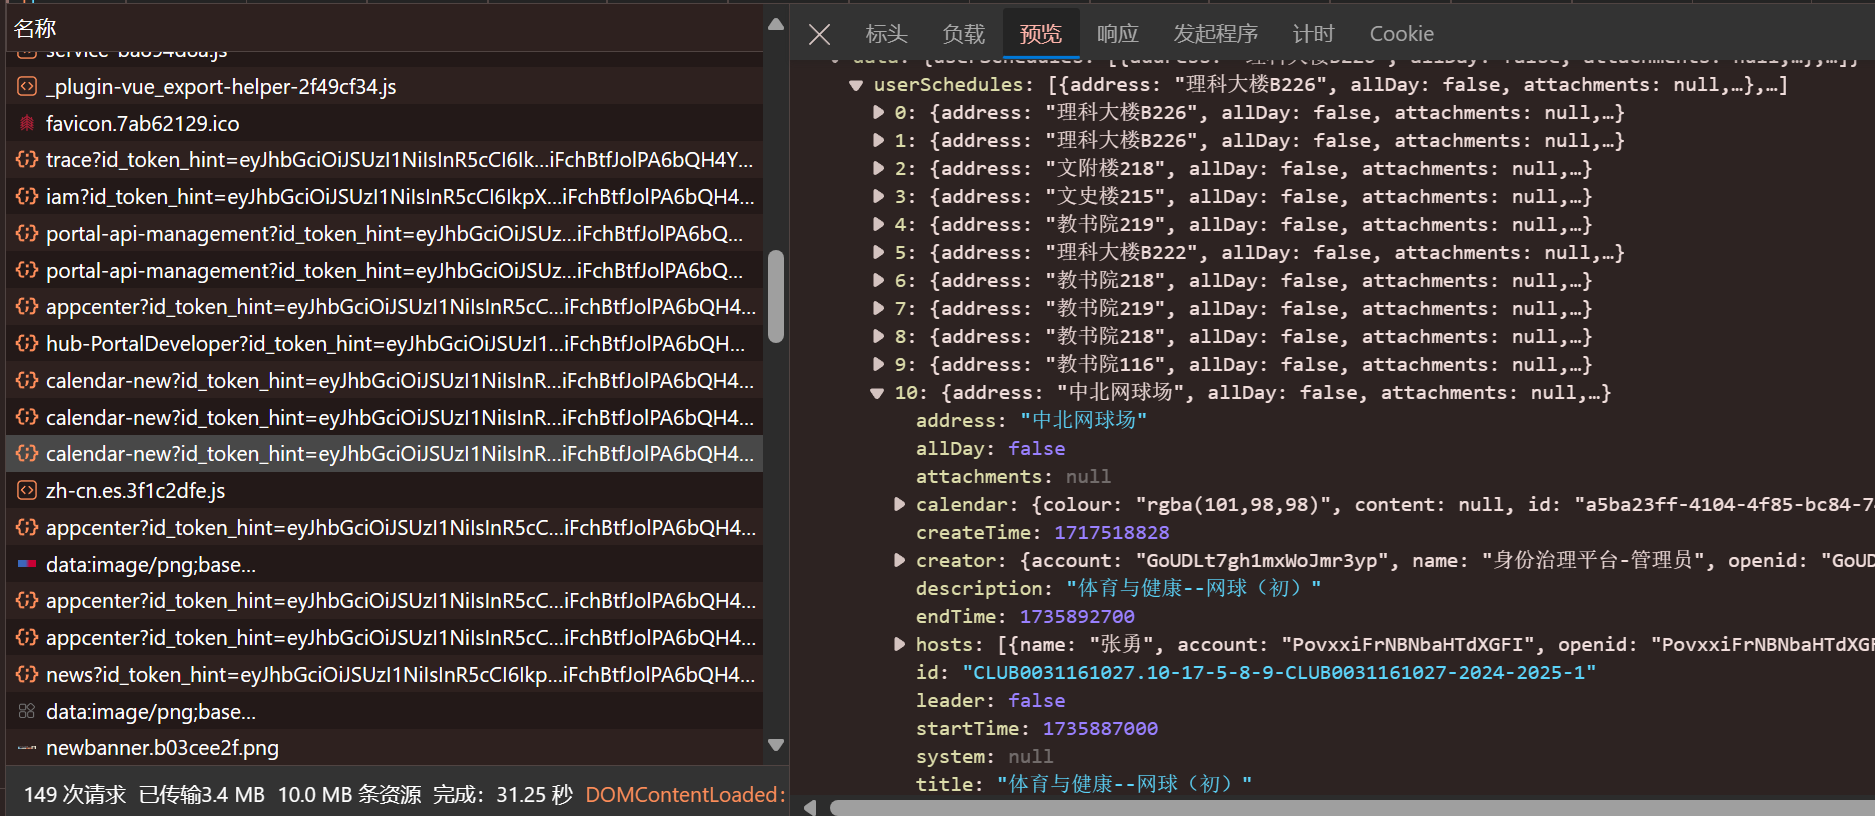
\includegraphics[width=0.8\textwidth]{img/calendar-new-url.png}
    \caption{Portal 课表请求}
    \label{fig:portal_course_table}
\end{figure}

这个 POST 请求采用的是 GraphQL 的查询格式,我们只需要使用 filter 过滤器查询自己所需要的字段即可。

\begin{lstlisting}[language=python]
    USER_SCHEDULES = """
    query ($filter: ScheduleFilter, $userId: String) {
      userSchedules(filter: $filter, userId: $userId) {
        address # 上课地点
        hosts {
          name # 教师名字
        }
        description # 课程信息和描述
        endTime # 结束时间
        startTime # 开始时间
      }
    }
    """
\end{lstlisting}

我们原定的设计是查询当前时刻至次日该时刻,用户的课程安排,如果有课程,上课前的一定时段发送邮件提醒用户去上课。
可以通过插件配置来配置上课前多久提醒用户,相关内容在后面进行详述。

\begin{rmr}
    该功能配置一次后,便可以在后台轮询调用,
    后续我们考虑加入手机端的定位功能,查询用户是否已经到达指定的上课地点,便不发送邮件。
\end{rmr}

    \subsection{测试模块}\label{subsec:tests}
    在本项目中,我们采用了 Python 标准库中的 \texttt{unittest} 模块进行单元测试,以确保项目核心功能的稳定性和正确性。

\begin{itemize}
    \item \textbf{测试环境的隔离}:通过 \texttt{setUp()} 和 \texttt{tearDown()} 方法,\texttt{unittest} 提供了对每个测试用例的独立初始化和资源回收,避免测试用例之间的相互干扰。
    \item \textbf{断言机制}:\texttt{unittest} 提供了多种断言方法(如 \texttt{assertEqual()}、\texttt{assertTrue()}),用以验证测试结果是否符合预期。
\end{itemize}

\textbf{测试用例的结构设计}:

以下是测试模块的代码结构:
\begin{lstlisting}[language=Python]
class TestCalendar(unittest.TestCase):
    def setUp(self):
        init()  # 初始化日志记录器
        self.cache = load_cache()  # 加载登录缓存
        self.calendar = CalendarQuery(self.cache.get_cache(PortalCache))

    def test_user_schedules(self):
        now = datetime.datetime.now()
        pprint(self.calendar.query_user_schedules(
            int(now.timestamp() * 1000),
            int((now + datetime.timedelta(days=1)).timestamp() * 1000),
        ))

    def test_school_calendar(self):
        school_calendar = self.calendar.query_school_calendar()
        pprint(school_calendar)
\end{lstlisting}

\textbf{测试框架的执行流程}:
\begin{itemize}
    \item 在 \texttt{setUp()} 方法中完成初始化工作,包括日志系统的初始化和登录缓存的加载。
    \item 使用 \texttt{test\_user\_schedules()} 方法测试用户日程的获取功能,通过时间戳计算和校验确保数据范围的准确性。
    \item 使用 \texttt{test\_school\_calendar()} 方法验证校历的查询功能,确保校历数据的完整性和准确性。
\end{itemize}


    \subsection{用户交互界面}\label{subsec:gui}
    \subsubsection{主页}

标题栏显示项目标题和登录状态,左侧是标签页切换按钮,右侧是主页大标题和登录、退出软件两个按钮,见图\ref{fig:home}。

\begin{figure}[H]
    \centering
    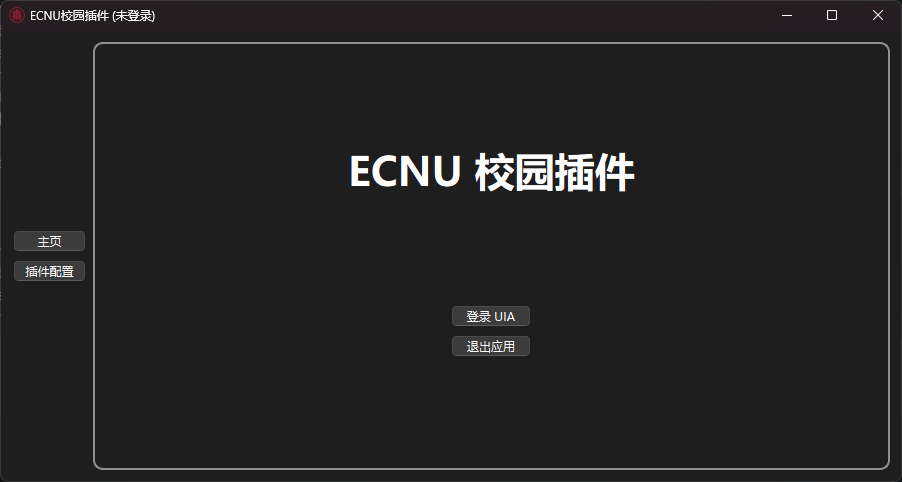
\includegraphics[width=0.8\textwidth]{img/home}
    \caption{主页}
    \label{fig:home}
\end{figure}

\subsubsection{插件配置页面}\label{subsubsec:gui-plugin-config}

插件配置页面右侧框中左侧的列表是插件选择,鼠标单击即可进入各个插件的配置界面,如图\ref{fig:plugin-config-gui} 中红框所示。

在每个插件的配置界面,会根据插件注册时提供的配置项生成可交互配置界面。

\begin{figure}[H]
    \centering
    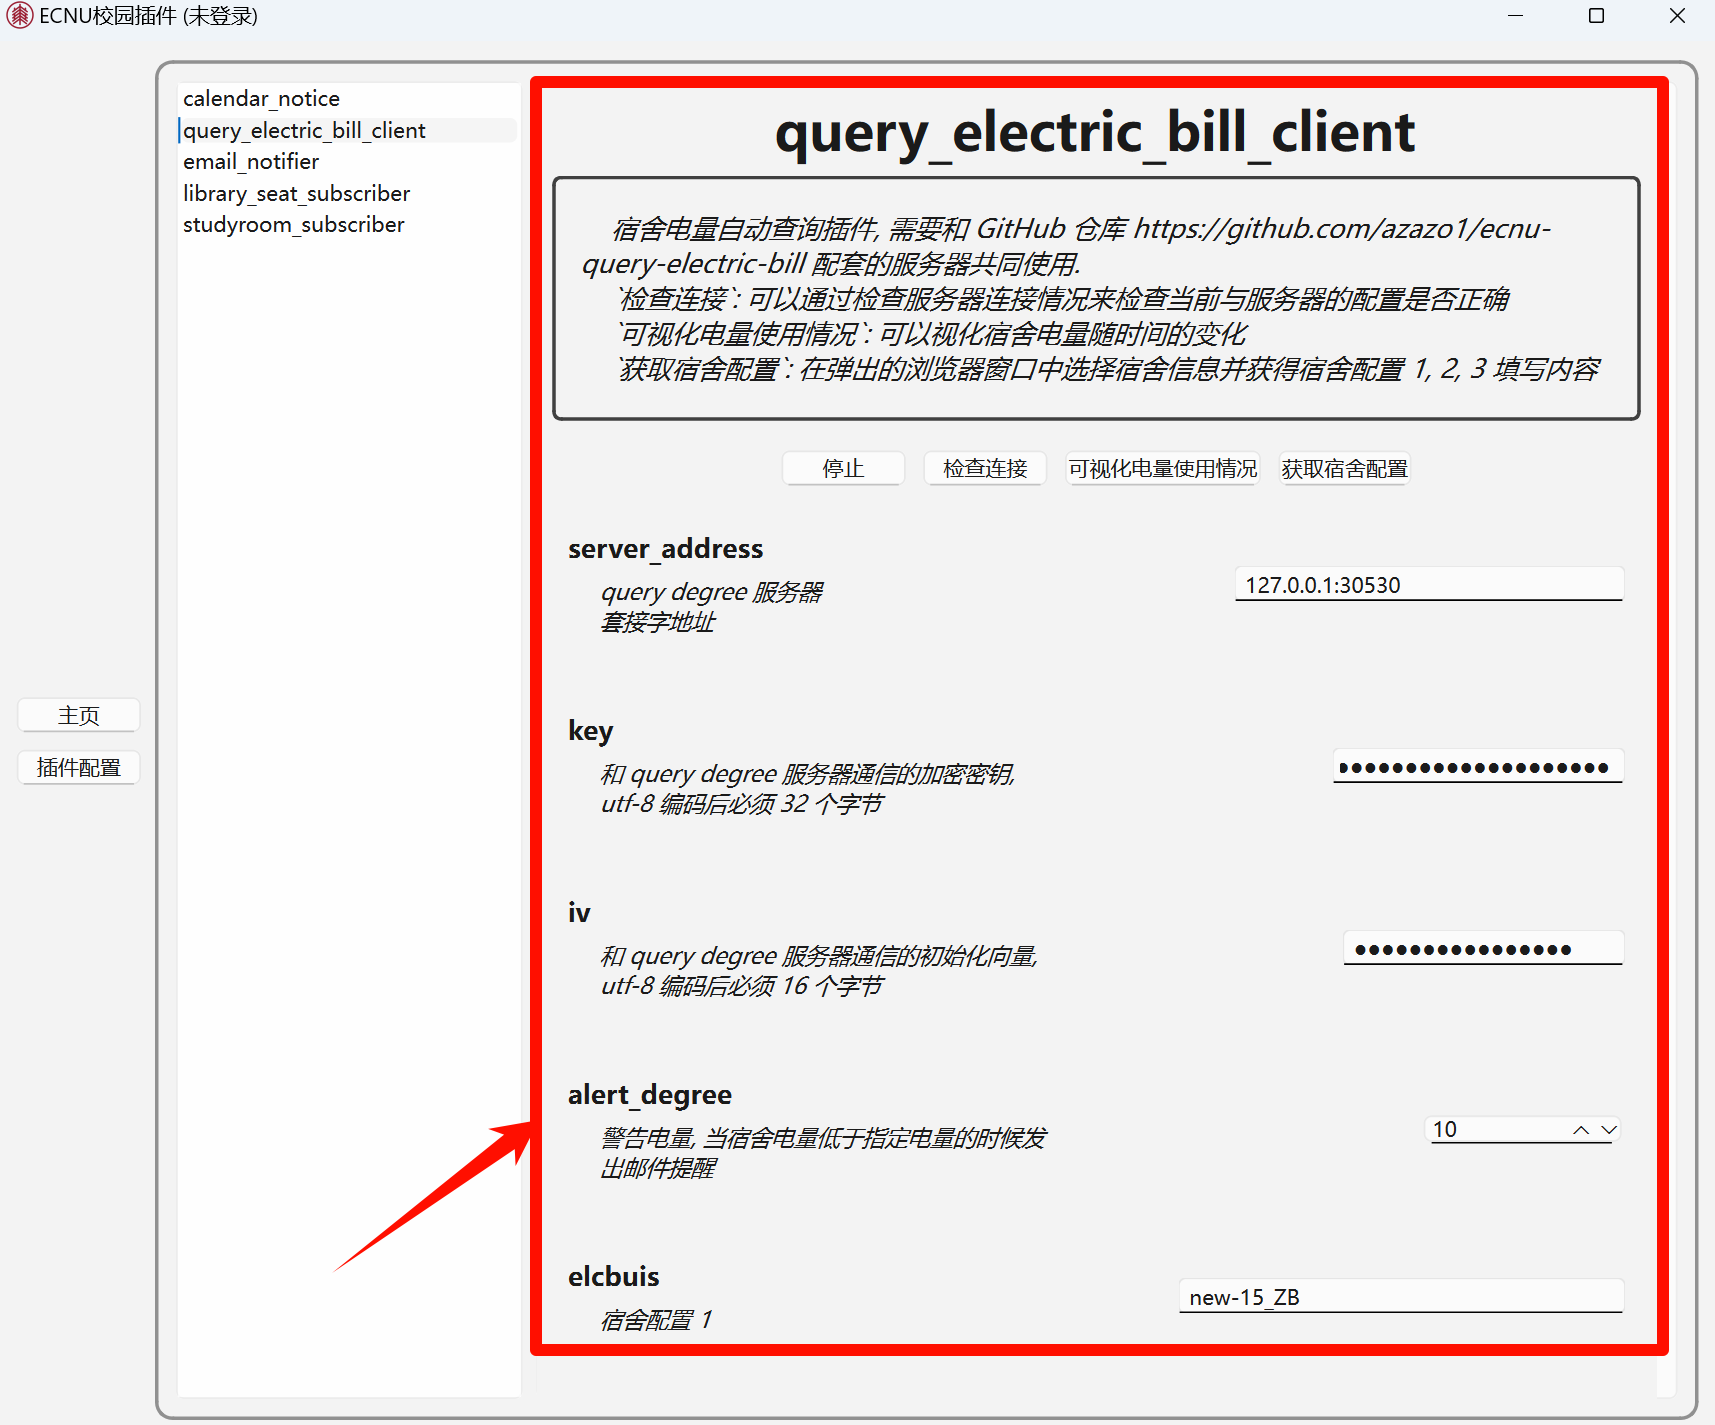
\includegraphics[width=0.8\textwidth]{img/plugin_config_gui}
    \caption{插件配置界面示例}
    \label{fig:plugin-config-gui}
\end{figure}

\subsubsection{系统托盘图标}

启动项目后,托盘中会出现 ECNU 图标,鼠标悬停可以查看当前的登录状态,使用鼠标右键显示菜单。
见图\ref{fig:tray-icon}、图\ref{fig:tray-icon-hover}、图\ref{fig:tray-icon-menu}。

\begin{figure}[H]
    \centering
    \begin{subfigure}[b]{0.3\textwidth}
        \centering
        
\includegraphics{img/tray_icon}
        \caption{系统托盘图标}
        \label{fig:tray-icon}
    \end{subfigure}
    \hspace{0.06\textwidth}
    \begin{subfigure}[b]{0.3\textwidth}
        \centering
        
\includegraphics{img/tray_icon_hover}
        \caption{鼠标悬浮显示状态}
        \label{fig:tray-icon-hover}
    \end{subfigure}
    \begin{subfigure}[b]{0.3\textwidth}
        \centering
        
\includegraphics{img/tray_icon_menu}
        \caption{右键显示菜单}
        \label{fig:tray-icon-menu}
    \end{subfigure}
\end{figure}



    \section{项目心得}\label{sec:thoughts}

    \begin{Thought}[关卓谦]
        在本项目中
    \end{Thought}

    \begin{Thought}[张梓卫]
        我是本项目的组织者和相关 Idea 的提出者,也是该课程报告的主要撰写人,
        得益于良好的团队框架,我能够马上上手研修间预约模块的开发,熟悉了数据处理和 API 调用的结合应用,
        当然,LateX 课表生成器的开发让我对编译有了更深入的理解,

        \vspace{0.3cm}

        在不断翻看 \verb`PluginLoader` 的代码到理解,最终写出一份详解的报告
        通过团队交流,我增强了自己的跨领域的开发编程能力,掌握了 Git 多种不同的使用方式,
        同时跟随团队的项目规范,掌握了如何通过良好的代码架构提高代码复用性和维护性。

        \vspace{0.3cm}

        同时,我还学到了如何利用 Python 的自动化工具(Selenium-Wire 和 requests)
        实现复杂的登录流程。翻看华东师范大学开发者文档时,涉及到鉴权,还了解到了 OAuth 2.0 和 JWT 等的认证机制。

        \vspace{0.3cm}

        是非常愉悦的一次项目经历!
    \end{Thought}

    \begin{Thought}[王文锦]
        在本项目中
    \end{Thought}

\end{document}